\documentclass[12pt,a4paper]{article}

\usepackage[utf8]{inputenc}
\usepackage[T2A,T1]{fontenc}
\usepackage[english,russian]{babel}

\usepackage[a4paper]{geometry} % showframe
\geometry{left=3cm}
\geometry{right=2cm}
\geometry{top=2cm}
\geometry{bottom=2cm}

\usepackage{amsmath}
\DeclareMathOperator{\Div}{div}
\DeclareMathOperator{\Rot}{rot}
\DeclareMathOperator{\sign}{sign}
\DeclareMathOperator{\TV}{TV}

\usepackage{amsfonts}
\usepackage{mathtools}
\usepackage{bm}
\usepackage{hyperref}
\usepackage[dvipsnames]{xcolor}

\usepackage{pgfplots}
\pgfplotsset{compat=1.9}

\usepackage{float}
\usepackage{commath}
\usepackage{xfrac}
%\usepackage{tempora}
\usepackage{indentfirst}

\usepackage[compact]{titlesec}
\newcommand{\sectionbreak}{\clearpage}

\titleformat{\section}{\normalfont\LARGE\bfseries}{\thesection.}{1em}{\setstretch{0.1}}
\titleformat{\subsection}{\normalfont\Large\bfseries}{\thesubsection.}{1em}{\setstretch{0.1}}
\titleformat{\subsubsection}{\normalfont\large\bfseries}{\thesubsubsection.}{1em}{}

\usepackage[shortlabels]{enumitem}
\usepackage{subcaption}
\usepackage{multirow}
\usepackage{setspace}

\usepackage{csquotes}
\usepackage [style=ieee, sorting=none, bibencoding=utf8, backend=biber, autolang=other, date=year, url=false,doi=false, isbn=false]{biblatex}
\addbibresource{ref.bib}

\newcommand\footnoteref[1]{\protected@xdef\@thefnmark{\ref{#1}}\@footnotemark}

\begin{document}

%\singlespacing
%%\pagestyle{empty}

\begin{titlepage}
    \begin{center}
        Федеральное государственное автономное образовательное учреждение
        
        высшего образования
        
        «Московский физико-технический институт
        
        (национальный исследовательский университет)»
        
        Физтех-школа Прикладной Математики и Информатики
        
        Кафедра информатики и вычислительной математики
    \end{center}

    \begin{flushleft}
        \textbf{Направление подготовки / специальность:} 03.03.01  Прикладные математика и физика (бакалавриат)\\
        
        \textbf{Направленность (профиль) подготовки:} Математическое моделирование, вычислительная математика и физика
    \end{flushleft}

    \begin{center}
        \vspace{\fill}
        \Large \bfseries
        КОМПЬЮТЕРНОЕ МОДЕЛИРОВАНИЕ ДИНАМИЧЕСКИХ ПРОЦЕССОВ В ИНДУСТРИАЛЬНЫХ ЛЕДОВЫХ КОНСТРУКЦИЯХ \vspace{1em}
        
        \normalsize \normalfont
        (бакалаврская работа)
        \vspace{\fill}
    \end{center}

    \hfill
    \begin{tabular}{@{}l@{}}
        \textbf{Студент:} \\
        Сергеев Фёдор Игоревич \\
        \medskip\\
        \hline\multicolumn{1}{c}{{\textit (подпись студента)}}\\
        \\
        \textbf{Научный руководитель:} \\
        Петров Игорь Борисович, \\
        чл.-корр. РАН, д. физ.-мат. наук, проф.\\
        \medskip\\
        \hline\multicolumn{1}{c}{{\textit (подпись руководителя)}}\\
        \\
        \textbf{Консультант} \textit{(при наличии)}\textbf{:} \\
        Хохлов Николай Игоревич, \\
        канд. физ.-мат. наук \\
        \medskip\\
        \hline\multicolumn{1}{c}{{\textit (подпись консультанта)}}
    \end{tabular}

    \vspace{2em}

    \begin{center}
        Москва \\
        2020
    \end{center}
\end{titlepage}

\onehalfspacing

\addtocounter{page}{1}
\thispagestyle{plain}
\begin{center}
    \LARGE
    \textbf{Аннотация}
\end{center}

Цель данной работы --- проведение компьютерного моделирования волновых процессов, происходящих при эксплуатации искусственных ледовых островов, а также исследование применения поглощающих граничных условий типа PML совместно с сеточно-характеристическим методом для задач вычислительной геофизики.

В рамках работы проведено моделирование распространения волн упругости в ледовом острове, воде и грунте при бурении; найдены распределения напряжений в ледовом острове при статической нагрузке и выявлены области острова, наиболее подверженные разрушению.

Также в данной работе была теоретически доказана возможность применения поглощающих граничных условий Bere\-nger PML и split-field PML совместно с сеточно-характеристическим методом для двумерной системы уравнений акустики. Для этих граничных условий проведён численный эксперимент по сравнению эффективности работы конечно-разностной и сеточно-харак\-теристической реализаций, показавший превосходство последних.

\newpage

\singlespacing
\tableofcontents
\onehalfspacing

\newpage

\section{Введение}

Арктический регион имеет огромные запасы полезных ископаемых. Например, суммарный объём одних только газовых месторождений на шельфе северных морей достигает 2.7 трлн тонн. Поиск, разработка и эксплуатация новых месторождений перспективны, но требуют решения новых вычислительных и инженерных задач для обеспечения эффективной и безопасной работы в Арктике \cite{petrov_arctic}.

В настоящее время особенный интерес для нефтегазовой индустрии представляет добыча полезных ископаемых на Арктическом шельфе с использованием искусственных ледовых островов. 

Ледовые острова обладают рядом преимуществ перед традиционными бетонными и металлическими нефтегазовыми платформами. Во-первых, основной строительный материал, лёд, в Арктике доступен и дёшев. Во-вторых, при использовании льда платформа является абсолютно экологически чистой. В третьих, в летний период лёд тает сам по себе, тем самым избавляя от необходимости проведения полного демонтажа несущих конструкций при завершении работы платформы. Это особенно важно для упрощения и удешевления разведочного бурения. Описанные преимущества делают ледовые острова отличным инструментом для проведения разведочного бурения в мелководных районах Северных морей.

При использовании ледовых островов возникает и ряд проблем. Важнейшей является обеспечение безопасности персонала и установок, находящихся на  поверхности острова. Устойчивости и целостности льда угрожают как механические, так и термические воздействия. К механическим воздействиям относятся сейсмическая активность \cite{ice_during_earthquake}, столкновение с айсбергами и ледовыми полями \cite{iceberg_crash, iceberg_crash2}, бурение и статическая нагрузка \cite{epifanov_crash}. К термическим --- воздействие солнечной радиации и тёплых течений  \cite{canadian_arctic, petrov_arctic}. Другой проблемой, возникающей при эксплуатации ледовых островов, оказывается значительное влияние льда на сейсморазведку \cite{stogniy_ice_influence}. Отражение упругих волн от поверхностей острова усложняет сейсмограммы, затрудняя их анализ и утяжеляя поиск полезных ископаемых.

Для расчёта механических воздействий, оказываемых на ледовый остров, требуется численное моделирование распространения упругих волн во льду и геологических средах. Для этих целей хорошо зарекомендовал себя  сеточно-характеристичес\-кий метод. С его помощью можно решать задачи как на прямоугольных, так и на тетраэдральных сетках. Это позволяет применять его для моделирования неоднородных и трещиноватых сред. К его достоинствам также относится возможность постановки корректных граничных и контактных условий. Кроме того, сеточно-характеристический метод эффективно распараллеливается, позволяя производить объёмные расчёты на многопроцессорных вычислительных системах.  \cite{petrov_arctic, zhdanov_gcm, biryukov_fractured_layers, favorskaya_thesis, grigoriev}

При моделировании распространения волн в геологических средах часто используются поглощающие граничные условия \cite{seismo_pml,arch_comp_sim}. Самым простым поглощающим условием , пожалуй, является граничное условие Mur \cite{arch_comp_sim}. Граничные условиями типа полностью согласованного слоя (PML) --- более сложные, но и более эффективные. Разработано множество вариантов граничных условий PML, в частности, Berenger PML \cite{berenger} и split-field PML \cite{split_field_pml}. Граничные условия Mur, Berenger PML и split-field PML используются, как правило, совместно с конечно-разностным методом. Интересно  изучить возможность их применения совместно с  сеточно-характеристическим методом.

Данная работа состоит из двух частей. В первой части рассмотрено компьютерное моделирование динамических процессов в ледовом острове, в том числе задача о бурении и статической нагрузке. Во второй части рассмотрены поглощающие граничные условия типа  Mur, Berenger PML и split-field PML для двумерной системы уравнений акустики, проведён анализ их эффективности при использовании конечно-разностного и сеточно-характеристического методов.

\section{Моделирование динамических процессов в ледовом острове}

\subsection{Постановка задачи}

Рассмотрим в двумерном случае ледовый остров шириной 300 м. и высотой 10 м., покоящийся на дне моря глубиной 8 м.

Грунт под островом будем считать состоящим из придонного слоя глубиной 10 м. и слоя осадочных пород глубиной 600 м. В некоторых случаях мы будем также рассматривать  газоносный слой, находящийся под слоем осадочных пород. Параметры рассматриваемых сред приведены в \autoref{tab:geo}.

Ставятся следующие задачи

\begin{enumerate}
    \item Исследовать распространение акустических и упругих волн от бура, расположенного посередине длины острова на глубине 20 м., с учётом наличия газоносного слоя (см. \autoref{fig:island}).
    
    \begin{figure}[htb]
        \centering
        \includegraphics[width=0.8\textwidth]{images/gas_field/gas_field_scheme.png}
        \caption{Постановка задачи о бурении.}
        \label{fig:island}
    \end{figure}

    \item Найти распределение напряжений в ледовом острове при наличии здания на поверхности острова (см. \autoref{fig:stamp_scheme})\footnote{Здесь линейные размеры совпадают с задачей о бурении, если не указано обратное.}. Оценить максимальную величину статической нагрузки, которая не приводит к разрушению льда. Найти области острова, наиболее подверженные разрушению.
    
    \begin{figure}[htb]
        \centering
        \includegraphics[width=0.8\textwidth]{images/stamp/stamp_scheme.png}
        \caption{Постановка задачи о статической нагрузке.}
        \label{fig:stamp_scheme}
    \end{figure}
\end{enumerate}

\renewcommand{\arraystretch}{1.2}
\begin{table}[htb]
\centering
    \begin{tabular}{|l|c|c|c|}
    \hline
    Среда & $c_p$, м/с & $c_s$, м/с & $\rho$, кг/м\textsuperscript{3} \\ \hline
    Лёд & 3940 & 2493 & 917 \\ \hline
    Вода & 1500  & --- & 1025 \\ \hline
    Придонный грунт & 1806 & 316 & 2000 \\ \hline
    Осадочные породы & 2250 & 1000 & 2000 \\ \hline
    \end{tabular}
\caption{Параметры рассматриваемых сред.}
\label{tab:geo}
\end{table}
\renewcommand{\arraystretch}{1.0}

\subsection{Математическая модель среды}

\subsubsection{Уравнения}

Рассматриваемые среды (см. таблицу \autoref{tab:geo}) будем считать сплошными, однородными, изотропными и несжимаемыми. В описанной постановке присутствуют как жидкие среды (вода, окружающая остров), так и твёрдые среды (лёд и слои грунта).

Жидкие среды в двумерном случае в декартовой эйлеровой системе координат описываются акустическим волновым уравнением

\begin{equation}
    \begin{dcases}
        \rho \frac{\partial \vec{v}(x,y,t)}{\partial t} = -\nabla p (x,y,t) \\
        \frac{\partial p(x,y,t)}{\partial t} = -\rho c^2 \Div \vec{v}(x,y,t)
    \end{dcases}
    \label{eq:acoustic_wave_eq}
\end{equation}

где $\rho$ --- плотность среды, $\vec{v}(x,y,t)$ --- вектор скорости (производная вектора смещения частицы среды $\vec{u}(x,y,t)$ по времени), $p(x,y,t)$ --- давление, $c$ --- скорость звука в жидкости.

Твёрдые среды в двумерном случае в декартовой эйлеровой системе координат описываются уже  упругим волновым уравнением
\begin{equation}
    \begin{dcases}
        \rho \frac{\partial \vec{v}(x,y,t)}{\partial t} = \Div^T \pmb{\sigma} (x,y,t) \\
        \frac{\partial \pmb{\sigma}(x,y,t)}{\partial t} = \rho \left(c_p^2 - 2c_s^2\right) \Div \vec{v}(x,y,t) \pmb{I} + \rho c_s^2 \left(\nabla \otimes \vec{v}(x,y,t) + \left[ \nabla \otimes \vec{v}(x,y,t)\right]^T \right)
    \end{dcases}
    \label{eq:elastic_wave_eq}
\end{equation}

где $\pmb{\sigma}(x,y,t)$ --- симметричный тензор напряжений Коши второго ранга, $c_p$ и $c_s$ --- скорости продольной и поперечной волн соответственно, $\pmb{I}$ --- единичный тензор второго ранга, операция $\otimes$ --- тензорное произведение векторов.

Далее для краткости мы будем опускать значок у вектора скорости, то есть будем писать $v$, подразумевая при этом вектор $\vec{v}$. Также мы будем опускать параметры $(x,y,t)$ у зависящих от них величин.

\subsubsection{Контактные условия}

Между средами необходимо поставить контактные условия, которые изображены на \autoref{fig:contacts} (они одинаковы для задачи о буре и задачи о статической нагрузке).

\begin{figure}[htb]
    \centering
    \includegraphics[width=0.8\textwidth]
    {images/gas_field/contacts.png}
    \caption{Схема контактных условий: 1 --- контактное условие полного слипания, 2 --- контактное условие между упругой и акустической средами, 3 --- контактное условие скольжения, 4 --- контактное условие отражения.}
    \label{fig:contacts}
\end{figure}

Здесь и далее мы будем обозначать контактирующие среды (или расчётные сетки) индексами $L$ и $R$ --- левая и правая среды соответственно. Вектор внешней нормали к левой под-области обозначим как $n$.

\begin{enumerate}
    \item Контактное условие полного слипания ставится между слоями твёрдых сред. Физически оно означает возможность беспрепятственного распространения упругих волн. Для этого требуется равенство скоростей и векторов нормального напряжения на границе раздела.
    
    Математически условие полного слипания записывается следующим образом
    \begin{equation}
    \begin{dcases}
        v_L = v_R \\
        \pmb{\sigma}_L \cdot n = \pmb{\sigma}_R \cdot n
    \end{dcases}
    \end{equation}
    
    \item Контактное условие между упругой и акустической средой используется для реализации перехода волн из твёрдых сред в жидкость и обратно. Оно отличается от условий полного слипания, т.к. в данном случае контактирующие среды описываются разными уравнениями (см. \eqref{eq:acoustic_wave_eq} и  \eqref{eq:elastic_wave_eq}).
    
    Если считать, что акустическая среда отвечает индексу $L$, а упругая --- $R$, то данное условие запишется как
    \begin{equation}
    \begin{dcases}
        v_L \cdot n = v_R \cdot n \\
        \pmb{\sigma} \cdot n + p n = 0
    \end{dcases}
    \end{equation}
    
    Физически это условие означает не-протекание жидкости в твёрдое тело, и наоборот. Для этого требуется равенство нормальных скоростей. первое уравнение, и равенство нормального вектора напряжений на контактной границе, второе уравнение.
    
    \item Контактное условие свободного скольжения ставится между ледовым островом и грунтом. В отличие от случая контакта двух слоёв грунта, когда применяется условие полного слипания, лёд и придонный слой могут двигаться друг относительно друга. Это явление известно на практике, так, например, наблюдается "соскальзывание" ледников с поверхностей гор. Таким образом требуется использование специального контактного условия.
    \begin{equation}
    \begin{dcases}
        v_L \cdot n = v_R \cdot n \\
        n \cdot \pmb{\sigma}_L \cdot n = n \cdot \pmb{\sigma}_L \cdot n \\
        n \cdot \sigma_{L/R} \cdot n = \sigma_{L/R} \cdot n
    \end{dcases}
    \end{equation}

    \item Контактное условие полного отражения (свободной границы) ставится на границе раздела осадочных пород и газоносного слоя. Применение такого условия не является вполне физически верным, однако для нашей задачи его применение вполне оправдано.

    \begin{equation}
        \pmb{\sigma} \cdot n = 0
    \end{equation}
\end{enumerate}

\subsubsection{Граничные условия}

Граничные условия области изображены на \autoref{fig:borders} для задачи о бурении и на \autoref{fig:stamp_scheme} для задачи о статической нагрузке.

\begin{figure}[htb]
    \centering
    \includegraphics[width=0.8\textwidth]
    {images/gas_field/border_conds.png}
    \caption{Схема граничных условий для задачи о бурении: a --- граничное условие поглощения, b --- граничное условие нулевого давления.}
    \label{fig:borders}
\end{figure}

\begin{figure}[htb]
    \centering
    \includegraphics[width=0.8\textwidth]
    {images/stamp/stamp_border.png}
    \caption{Схема граничных условий для задаче о статической нагрузке: a --- граничное условие поглощения, b --- граничное условие нулевого давления, с --- граничное условие постоянного  давления.}
    \label{fig:stamp_borders}
\end{figure}

\begin{enumerate}[a.]
    \item Поглощающие (не-отражающие) граничные условия используются при рассмотрении ограниченной под-области бесконечного физического региона. В данном случае водяной, придонный, газоносный слои и слой осадочных пород продолжаются за границы расчётной области налево, направо и, для газоносного слоя, вниз. Поэтому на их краях необходимо использовать поглощающие граничные условия. \footnote{Поглощающие условия будут рассмотрены подробнее в главе \ref{sec:absorbing}.}
    
    Для упругих сред это условие запишется в виде
    
    \begin{equation}
    \begin{dcases}
        v_{l-2}^n = 
        v_{l-1}^n = 
        v_{l}^n \\
        \pmb{\sigma}_{l-2}^n = 
        \pmb{\sigma}_{l-1}^n = 
        \pmb{\sigma}_{l}^n
    \end{dcases}
    \end{equation}
    
    А для акустических сред в виде
    
    \begin{equation}
    \begin{dcases}
        v_{l-2}^n = 
        v_{l-1}^n = 
        v_{l}^n \\
        p_{l-2}^n = 
        p_{l-1}^n = 
        p_{l}^n
    \end{dcases}
    \end{equation}
    
    здесь верхний индекс $n$ обозначает момент времени $t_n$, а нижний --- номер сеточного узла, при этом узел $l$ является граничным, а узлы $l-1$ и $l-2$ --- его соседями по одной из осей. Такая форма записи будет верна для левой, правой и нижней границе при соответствующем выборе значений координатных индексов.
    
    \item Граничное условие нулевого давления применяется на границе сред с воздухом. В нашей задаче мы не учитываем влияние атмосферного давления на исследуемые процессы, считая его пренебрежимо малым. Следовательно мы принимаем $p=0$ на границах вода-воздух и лёд-воздух.
    
    \item Граничное условие постоянного давление задаёт давление здание на поверхность льда  $p=P_0$, не зависящее от времени.
\end{enumerate}

\subsection{Численный метод}

\subsubsection{Сеточно-характеристический метод}
\label{sec:elastic_gcm}

Для решения систем уравнений в частных производных \eqref{eq:elastic_wave_eq} и \eqref{eq:acoustic_wave_eq} воспользуемся сеточно-характеристическим методом на регулярных прямоугольных сетках. Получим его для системы \eqref{eq:acoustic_wave_eq}, описывающей упругие среды. Для системы \eqref{eq:acoustic_wave_eq} он получается абсолютно аналогично если учесть, что для акустических сред $\sigma_{xx} = \sigma_{yy} = p$ и $\sigma_{xy}=0$.

Будем работать в декартовой прямоугольной системе координат. Введём обозначение 
\begin{equation}
    \varphi = \begin{pmatrix} v_x \\ v_y \\ \sigma_{xx} \\ \sigma_{xy} \\ \sigma_{yy} \end{pmatrix}
\end{equation}

Нижние индексы здесь обозначают соответствующие компоненты вектора скорости $v$ и тензора напряжений $\pmb{\sigma}$.

Запишем гиперболическую полную систему линейный дифференциальных уравнений в частных производных \eqref{eq:elastic_wave_eq} в канонической матричной форме

\begin{equation}
    \dfrac{\partial \varphi}{\partial t} + 
    \pmb{A} \dfrac{\partial \varphi}{\partial x} + 
    \pmb{B} \dfrac{\partial \varphi}{\partial y} = 0
\end{equation}

\begin{equation}
    \pmb{A} = \begin{pmatrix}
        0 & 0 & -\frac{1}{\rho} & 0 & 0 \\
        0 & 0 & 0 & -\frac{1}{\rho} & 0 \\
        -(\lambda+2\mu) & 0 & 0 & 0 & 0 \\
        0 & -\mu & 0 & 0 & 0 \\
        -\lambda & 0 & 0 & 0 & 0
    \end{pmatrix}
\end{equation}

\begin{equation}
    \pmb{B} = \begin{pmatrix}
        0 & 0 & 0 & 0 & 0 \\
        0 & 0 & -\frac{1}{\rho} & 0 & 0 \\
        0 & -\lambda & 0 & 0 & 0 \\
        -\mu & 0 & 0 & 0 & 0 \\
        0 & -(\lambda+2\mu) & 0 & 0 & 0
    \end{pmatrix}
\end{equation}

Здесь $\lambda$ и $\mu$ --- параметры Ламе, которые выражаются через заданные для конкретных сред скорости продольных и поперечных волн

\begin{equation}
    \begin{dcases}
        c_p = \sqrt{\dfrac{\lambda + 2\mu}{\rho}} \\
        c_s = \sqrt{\dfrac{\mu}{\rho}}
    \end{dcases}
\end{equation}

\begin{equation}
    \begin{dcases}
        \lambda = \left(c_p^2 - 2 c_s^2\right) \rho \\
        \mu = c_s^2 \rho
    \end{dcases}
\end{equation}

Используя метод расщепления для системы, записанной в каноническом виде, получим систему

\begin{equation}
    \begin{dcases}
        \dfrac{\partial \varphi_x}{\partial t} + \pmb{A} \dfrac{\partial \varphi_x}{\partial x} = 0 \\
        \dfrac{\partial \varphi_y}{\partial t} + \pmb{B} \dfrac{\partial \varphi_y}{\partial y} = 0
    \end{dcases}
    \label{eq:rashepl_elastic}
\end{equation}

Заметим, что матрицы $\pmb{A}$ и $\pmb{B}$ можно диагонализовать
%https://www.wolframalpha.com/input/?i=%7B%7B0%2C0%2C-1%2Fp%2C0%2C0%7D%2C%7B0%2C0%2C0%2C-1%2Fp%2C0%7D%2C%7B-%28l%2B2m%29%2C0%2C0%2C0%2C0%7D%2C%7B0%2C-m%2C0%2C0%2C0%7D%2C%7B-l%2C0%2C0%2C0%2C0%7D%7D
%https://www.wolframalpha.com/input/?i=%7B%7B0%2C0%2C0%2C-1%2Fp%2C0%7D%2C%7B0%2C0%2C0%2C0%2C-1%2Fp%7D%2C%7B0%2C-l%2C0%2C0%2C0%7D%2C%7B-m%2C0%2C0%2C0%2C0%7D%2C%7B0%2C-%28l%2B2m%29%2C0%2C0%2C0%7D%7D

\begin{gather*}
    \pmb{A} = \pmb{S}^{-1}_1 \pmb{\Lambda}_1 \pmb{S}_1 \\
    \pmb{B} = \pmb{S}^{-1}_2 \pmb{\Lambda}_2 \pmb{S}_2
\end{gather*}
\begin{gather*}
    \pmb{S}^{-1}_1 = 
    \begin{pmatrix}
        0 & 0 & 0 & \sqrt{\frac{\lambda + 2\mu}{\lambda^2 \rho}} & -\sqrt{\frac{\lambda + 2\mu}{\lambda^2 \rho}} \\
        0 & \frac{1}{\sqrt{\mu\rho}} & -\frac{1}{\sqrt{\mu\rho}} & 0 & 0 \\
        0 & 0 & 0 & \frac{2\mu}{\lambda} + 1 & \frac{2\mu}{\lambda} + 1 \\
        0 & 1 & 1 & 0 & 0 \\
        1 & 0 & 0 & 1 & 1
    \end{pmatrix}
    \quad
    \pmb{S}_1 = 
    \begin{pmatrix}
        0 & 0 & 0 & 0 & 1 \\
        0 & \frac{\sqrt{\mu\rho}}{2} & 0 & \frac{1}{2} & 0 \\
        0 & -\frac{\sqrt{\mu\rho}}{2} & 0 & \frac{1}{2} & 0 \\
        \sqrt{\frac{\lambda^2 \rho}{4\left(\lambda+2\mu\right)}} & 0 & \frac{\lambda}{2\lambda + 4\mu} & 0 & 0 \\
        -\sqrt{\frac{\lambda^2 \rho}{4\left(\lambda+2\mu\right)}} & 0 & \frac{\lambda}{2\lambda + 4\mu} & 0 & 0
    \end{pmatrix}
\end{gather*}
\begin{gather*}
    \pmb{S}^{-1}_2 = 
    \begin{pmatrix}
        0 & \frac{1}{\mu\rho} & -\frac{1}{\mu\rho} & 0 & 0 \\
        0 & 0 & 0 & \frac{1}{\sqrt{\left(\lambda+2\mu\right)\rho}} & -\frac{1}{\sqrt{\left(\lambda+2\mu\right)\rho}} \\
        1 & 0 & 0 & \frac{\lambda}{\lambda+2\mu} & \frac{\lambda}{\lambda+2\mu} \\
        0 & 1 & 1 & 0 & 0 \\
        0 & 0 & 0 & 1 & 1
    \end{pmatrix}
    \quad
    \pmb{S}_2 = 
    \begin{pmatrix}
        0 & 0 & 0 & 0 & 1 \\
        0 & \frac{\sqrt{\mu\rho}}{2} & 0 & \frac{1}{2} & 0 \\
        0 & -\frac{\sqrt{\mu\rho}}{2} & 0 & \frac{1}{2} & 0 \\
        \sqrt{\frac{\lambda^2 \rho}{4\left(\lambda+2\mu\right)}} & 0 & \frac{\lambda}{2\lambda + 4\mu} & 0 & 0 \\
        -\sqrt{\frac{\lambda^2 \rho}{4\left(\lambda+2\mu\right)}} & 0 & \frac{\lambda}{2\lambda + 4\mu} & 0 & 0
    \end{pmatrix}
\end{gather*}
\begin{gather*}
    \pmb{\Lambda}_1 = \pmb{\Lambda}_2 = 
    \begin{pmatrix}
        0 & 0 & 0 & 0 & 0\\
        0 & -\sqrt{\frac{\mu}{\rho}} & 0 & 0 & 0\\
        0 & 0 & \sqrt{\frac{\mu}{\rho}} & 0 & 0\\
        0 & 0 & 0 & -\sqrt{\frac{\lambda + 2\mu}{\rho}} & 0\\
        0 & 0 & 0 & 0 & \sqrt{\frac{\lambda + 2\mu}{\rho}}
    \end{pmatrix} = 
    \begin{pmatrix}
        0 & 0 & 0 & 0 & 0 \\
        0 & -c_s & 0 & 0 & 0 \\
        0 & 0 & c_s & 0 & 0 \\
        0 & 0 & 0 & -c_p & 0 \\
        0 & 0 & 0 & 0 & c_p
    \end{pmatrix}
\end{gather*}

Домножим слева первое уравнение системы \eqref{eq:rashepl_elastic} на $S_1$  а второе --- на $S_2$, при этом диагонализуя матрицы $\pmb{A}$ и $\pmb{B}$.

\begin{equation*}
\begin{dcases}
    \pmb{S}_1  \dfrac{\partial \varphi_x}{\partial t} +
    \pmb{S}_1 \left(\pmb{S}^{-1}_1 \pmb{\Lambda}_1 \pmb{S}_1 \right) \dfrac{\partial \varphi_x}{\partial x} = 0 \\
    \pmb{S}_2 \dfrac{\partial \varphi_y}{\partial t} + 
    \pmb{S}_2  \left(\pmb{S}^{-1}_2 \pmb{\Lambda}_2 \pmb{S}_2\right) \dfrac{\partial \varphi_y}{\partial y} = 0
\end{dcases}
\end{equation*}

Пользуясь тем, что матрицы $\pmb{S}_1$ и $\pmb{S}_2$ не зависят ни от времени, ни от координаты, вносим их в частные производные по времени и пространственным координатам 

\begin{equation*}
\begin{dcases}
    \dfrac{\partial}{\partial t} \left(\pmb{S}_1 \varphi_x\right) +
    \pmb{\Lambda}_1 \dfrac{\partial}{\partial x} \left(\pmb{S}_1 \varphi_x\right) = 0 \\
    \dfrac{\partial}{\partial t} \left(\pmb{S}_2 \varphi_y\right) + 
    \pmb{\Lambda}_2 \dfrac{\partial}{\partial y} \left(\pmb{S}_2 \varphi_y\right) = 0
\end{dcases}
\end{equation*}

Производя замену (переход к инвариантам Римана)

\begin{equation}
\begin{matrix}
    \omega_1 = \pmb{S}_1 \varphi_x \\
    \omega_2 = \pmb{S}_2 \varphi_y
\end{matrix}
\label{eq:riman_variable}
\end{equation}

получаем систему

\begin{equation}
\begin{dcases}
    \dfrac{\partial \omega_1}{\partial t}  +
    \pmb{\Lambda}_1 \dfrac{\partial \omega_1}{\partial x} = 0 \\
    \dfrac{\partial \omega_2}{\partial t} + 
    \pmb{\Lambda}_2 \dfrac{\partial \omega_2}{\partial y} = 0
\end{dcases}
\label{eq:grid_char_res}
\end{equation}

Произведённая замена \eqref{eq:riman_variable} очевидно обратимая, так как матрицы $\pmb{S}_i$, $i=1,2$ обратимы

\begin{equation}
\begin{matrix}
    \varphi_x  = \pmb{S}_1^{-1} \omega_1  \\
    \varphi_y  = \pmb{S}_2^{-1} \omega_2
\end{matrix}
\label{eq:riman_variable_inverse}
\end{equation}

Так как матрицы $\pmb{\Lambda}_i$ $i=1,2$ диагональные, то система \eqref{eq:grid_char_res} представляет собой 10 независимых скалярных уравнений переноса.

Таким образом общая схема решения систем \eqref{eq:elastic_wave_eq} и \eqref{eq:acoustic_wave_eq} следующая

\begin{enumerate}
    \item Произвести переход к инвариантам Римана \eqref{eq:riman_variable}.
    \item Решить систему независимых одномерных линейных уравнений переноса \eqref{eq:grid_char_res}.
    \item Осуществить обратный переход к физическим переменным \eqref{eq:riman_variable_inverse}.
\end{enumerate}

Заметим, что выбор метода решения одномерного уравнения переноса является открытым. При этом именно он определяет порядок аппроксимации всего сеточно-характеристического численного метода. Приведём несколько наиболее часто используемых схем для решения одномерного линейное уравнение переноса на скалярную величину $q$

\begin{equation}
    \dfrac{\partial q}{\partial t} + \lambda \dfrac{\partial q}{\partial x} = 0 \quad \lambda =const
    \label{eq:lin_advection}
\end{equation}

Также будем использовать запись этого уравнения через поток $f$

\begin{equation}
\begin{gathered}
    \dfrac{\partial q}{\partial t} + \dfrac{\partial f (u)}{\partial x} = 0 \\
    f = \lambda u
\end{gathered}
\label{eq:lin_advection_flux}
\end{equation}

\subsubsection{Схема Куранта-Изаксона-Риса}
%Courant, Richard; Isaacson, E; Rees, M. (1952). "On the Solution of Nonlinear Hyperbolic Differential Equations by Finite Differences". Comm. Pure Appl. Math. 5 (3): 243..255. doi:10.1002/cpa.3160050303.

\begin{figure}[htb]
    \centering
    \includegraphics[trim={55pt 100pt 530pt 100pt},clip,height=4cm]{images/theory/scheme_cir.png}
    \caption{Шаблон схемы Куранта-Изаксона-Риса.}
    \label{fig:scheme_cir}
\end{figure}

Схема Куранта-Изаксона-Риса для решения уравнения \eqref{eq:lin_advection} определяется как \cite{cir_scheme} \cite{petrov_lobanov_book}

\begin{equation*}
\begin{dcases}
    \dfrac{q_i^{n+1} - q_i^n}{\tau} + \lambda\dfrac{q_i^n - q_{i-1}^n}{h} = 0 & , \lambda > 0\\
    \dfrac{q_i^{n+1} - q_i^n}{\tau} + \lambda\dfrac{q_{i+1}^n - q_i^n}{h} = 0  & , \lambda < 0
\end{dcases}
\end{equation*}

Данная схема имеет первый порядок аппроксимации по времени и по пространству и является устойчивой при выполнении условия Куранта-Фридрихса-Леви

\begin{equation}
    C = \abs{\dfrac{\lambda \tau}{h}} \leq 1 
    \label{eq:cfl_condition}
\end{equation}

\subsubsection{Схема Русанова}
%К. М. Магомедов, А. С. Холодов, О построении разностных схем для уравнений гиперболического типа на основе характеристических соотношений, Ж. вычисл. матем. и матем. физ., 1969, том 9, номер 2, 373–386
%http://www.mathnet.ru/links/2f4d9e5725a56dabadced5481c2ca461/zvmmf7067.pdf
%https://www.intuit.ru/studies/courses/1170/213/lecture/5493?page=4

\begin{figure}[H]
    \centering
    \includegraphics[trim={55pt 100pt 35pt 100pt},clip,height=4cm]{images/theory/scheme_rusanov.png}
    \caption{Шаблон схемы Русанова третьего порядка аппроксимации.}
    \label{fig:scheme_rusanov}
\end{figure}

Схема Русанова использует промежуточные индексы и состоит из трёх этапов \cite{kholodov} \cite{petrov_lobanov_book}

\begin{enumerate}
    \item Переход $t_n \rightarrow t_{n+\sfrac{1}{3}}$ производится по схеме Лакса
    \begin{equation}
    \begin{gathered}
        \dfrac{q^{n+\sfrac{1}{3}}_{i+\sfrac{1}{2}} - \frac{1}{2}\left(q^n_i + q^n_{i+1}\right)}{\sfrac{\tau}{3}} + \dfrac{f^n_{i+1} - f^n_{i}}{h} = 0 \\
        \dfrac{q^{n+\sfrac{1}{3}}_{i-\sfrac{1}{2}} - \frac{1}{2}\left(q^n_i + q^n_{i-1}\right)}{\sfrac{\tau}{3}} + \dfrac{f^n_{i+1} - f^n_{i}}{h} = 0
    \end{gathered}
   \end{equation}
 
    \item Для шага $t_{n+\sfrac{1}{3}} \rightarrow t_{n+\sfrac{2}{3}}$ используется схема <<чехарда>>
    \begin{equation}
        \dfrac{q^{n+\sfrac{2}{3}}_{i} - q^n_i}{\sfrac{2\tau}{3}} + \dfrac{f^{n+\sfrac{1}{3}}_{i+\sfrac{1}{2}} - f^{n+\sfrac{1}{3}}_{i-\sfrac{1}{2}}}{h} = 0
    \end{equation}

    \item Последний шаг $t_{n+\sfrac{2}{3}} \rightarrow t_{n+1}$ следующий
    \begin{equation}
    \begin{gathered}
        \dfrac{q^{n+1}_i - q^n_i}{\tau} + \dfrac{3}{8}\dfrac{f^{n+\sfrac{2}{3}}_{i+1} - f^{n+\sfrac{2}{3}}_{i-1}}{h} + \dfrac{-2f^n_{i+2} + 7f^n_{i+1} -  7f^n_{i-1} +22f^n_{i-2}}{24h} +\\+ \dfrac{\omega}{24}\left(q^n_{i+2}-  4q^n_{i+1} + 6q^n_{i} - 4 q^n_{i-1} + q^n_{i-2}\right) = 0
    \end{gathered}
    \end{equation}
    
    Последнее слагаемое необходимо для обеспечения устойчивости данной схемы.
\end{enumerate}

Схема Русанова имеет третий порядок аппроксимации и является условно устойчивой при выполнении, в дополнении к условию Куранта-Фридрихса-Леви \eqref{eq:cfl_condition}, неравенства $4s^2 - s^4 \leq \omega \leq 3$, где $s = \frac{\tau}{h}$.

\subsubsection{Схема TVD 2-го порядка аппроксимации}

TVD-схемы позволяют решать задачи с большими градиентами, избегая появления осцилляций, вызванных дискретизацией задачи \cite{harten} \cite{rus_tvd} \cite{petrov_lobanov_book}. 

Полная вариация (total variation) решения линейного уравнения переноса \eqref{eq:lin_advection} определяется как

\begin{equation*}
    \TV \left(q(\cdot, t)\right) = \int \abs{\dfrac{\partial q}{\partial x}} dx
\end{equation*}

Соответственно полная вариация численного решения 

\begin{equation*}
    \TV \left(q^n\right) = \TV \left(q(\cdot, t^n)\right) = \sum_i \left| q_{i+1}^n - q_i^n \right|
\end{equation*}

Схема называется схемой с уменьшением полной вариации, или TVD-схемой (total variation diminishing scheme), или схемой, монотонной по Хартену, если

\begin{equation*}
    \TV \left(q^{n+1}\right) \leq \TV \left(q^n\right)
\end{equation*}

В некоторых расчётах мы будем использовать TVD-схему 2-го порядка

\begin{equation}
\begin{gathered}
    q_i^{n+1} = q_i^n - \dfrac{\tau}{h}\left(f_{i+\sfrac{1}{2}} - f_{i-\sfrac{1}{2}}\right) \\
    f_{i+\sfrac{1}{2}} = \dfrac{f_i^n + f^n_{i+1}}{2} - \dfrac{\theta}{2}\left(f_{i+1}^n - f_i^n\right) + \dfrac{\phi_{sb}(r_i)}{2} \left(\theta - C\right) \left(f_{i+1}^n - f_i^n\right) \\
    \theta = \sign C_{i+\sfrac{1}{2}}
\end{gathered}
\label{eq:tvd_scheme}
\end{equation}

с ограничителем superbee
\begin{equation}
    \phi_{sb}(r_i) = \max \left\{0, \min\{2r_i,1\}, \min\{r_i,2\}\right\}
\end{equation}

где
\begin{equation*}
    r_i = \dfrac{q_i - q_{i-1}}{q_{i+1} - q_i}
\end{equation*}

\subsection{Моделирование воздействия бура}

Современные буры имеют довольно сложное устройство, зачастую сочетая ударные и вращательные механизмы. В данной работе нас в первую очередь интересует волновая картина, возникающая при бурении в конкретной геологической модели (см. рис. \autoref{fig:island}). Поэтому, для простоты, воздействие бура мы будет представлять в качестве точечного источника давления в виде импульса Рикера частотой 30 Гц.
\begin{equation}
    p(x,y) = \dfrac{1}{\pi \sigma^4} \left(1-\dfrac{1}{2}\left(\dfrac{x^2+y^2}{\sigma^2}\right)\right) \exp\left({-\frac{x^2+y^2}{2\sigma^2}}\right)
    \label{eq:ricker}
\end{equation}

\begin{figure}[htb]
    \centering
    \includegraphics[trim={0pt 45pt 0pt 80pt},clip,width=0.7\textwidth]{images/gas_field/ricker_wavelet.png}
    \caption{График импульса Рикера \eqref{eq:ricker} при $\sigma=1$.}
    \label{fig:ricker_plot}
\end{figure}

\begin{figure}[H]
    \centering
    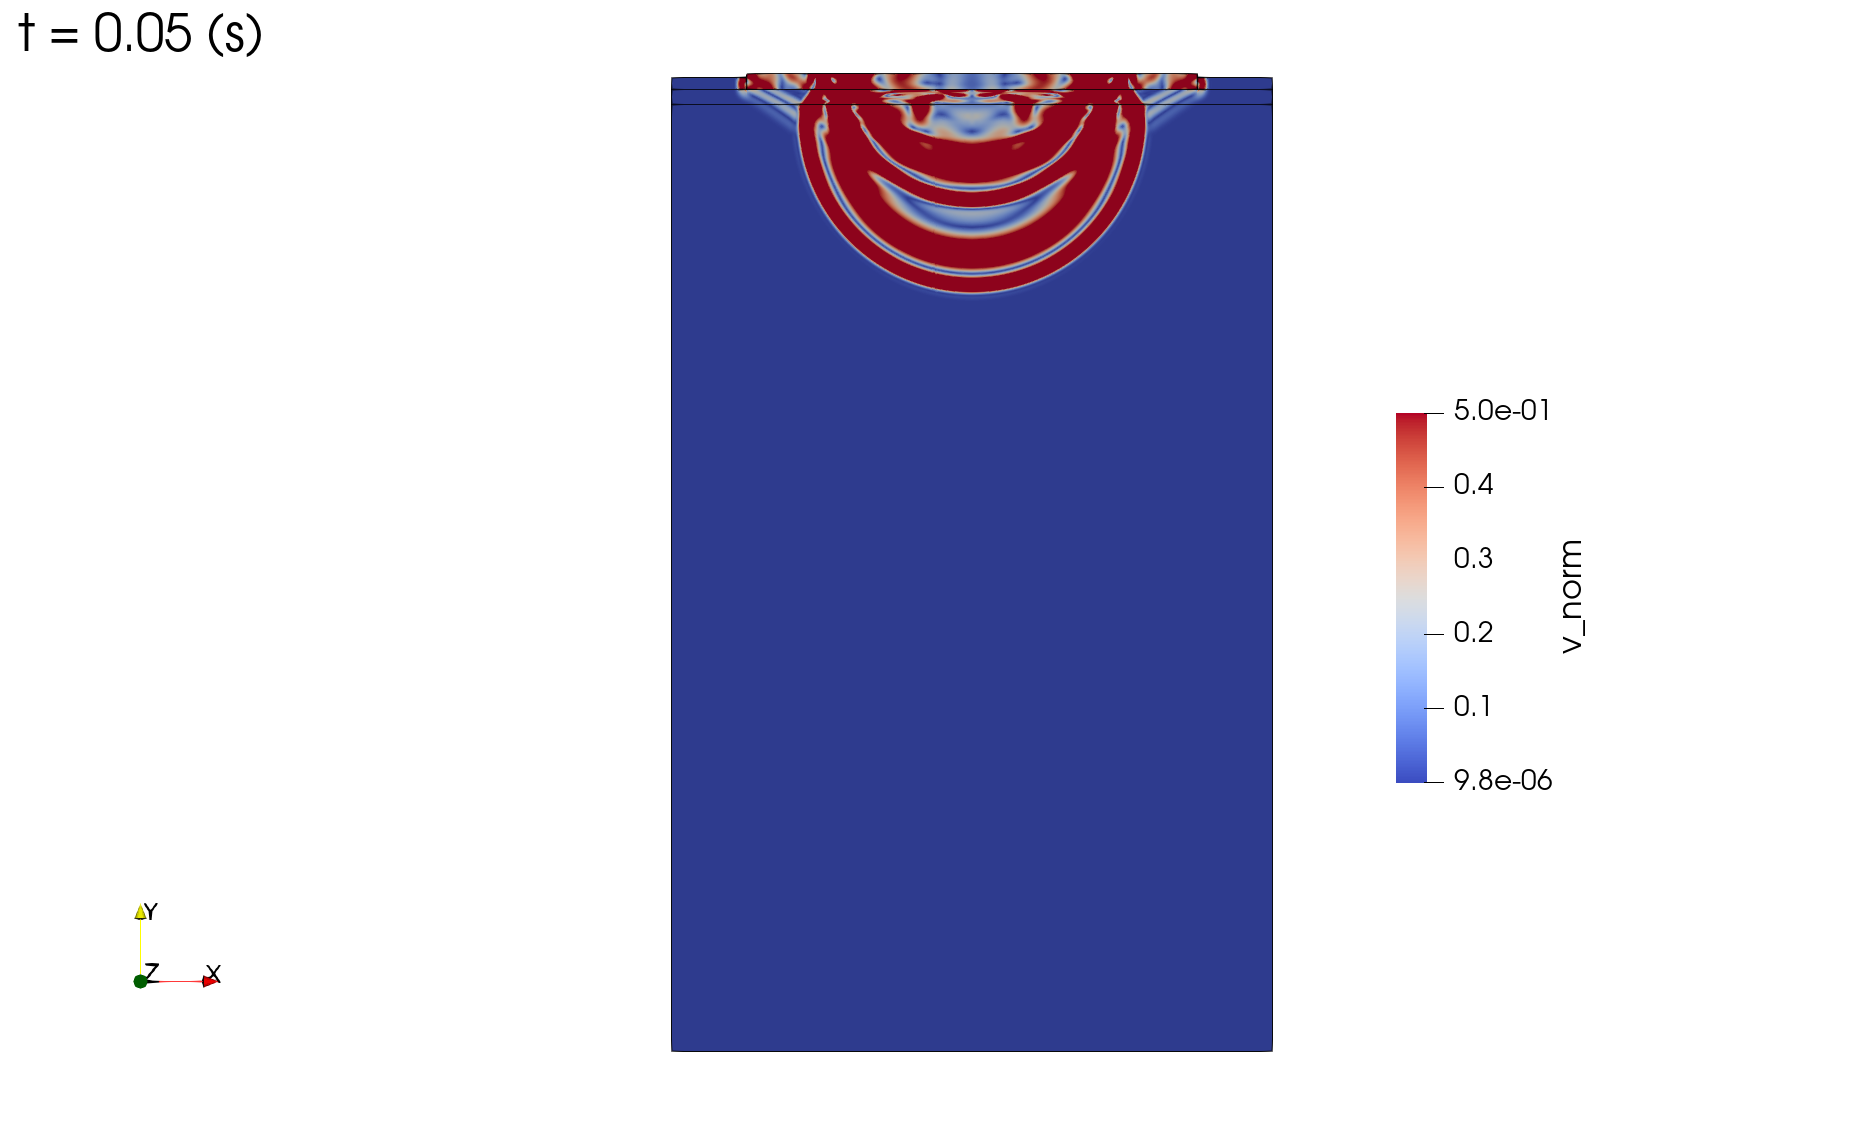
\includegraphics[trim={20cm 1cm 20cm 3cm},clip,width=0.32\textwidth]
    {images/gas_field/0.05.png}
    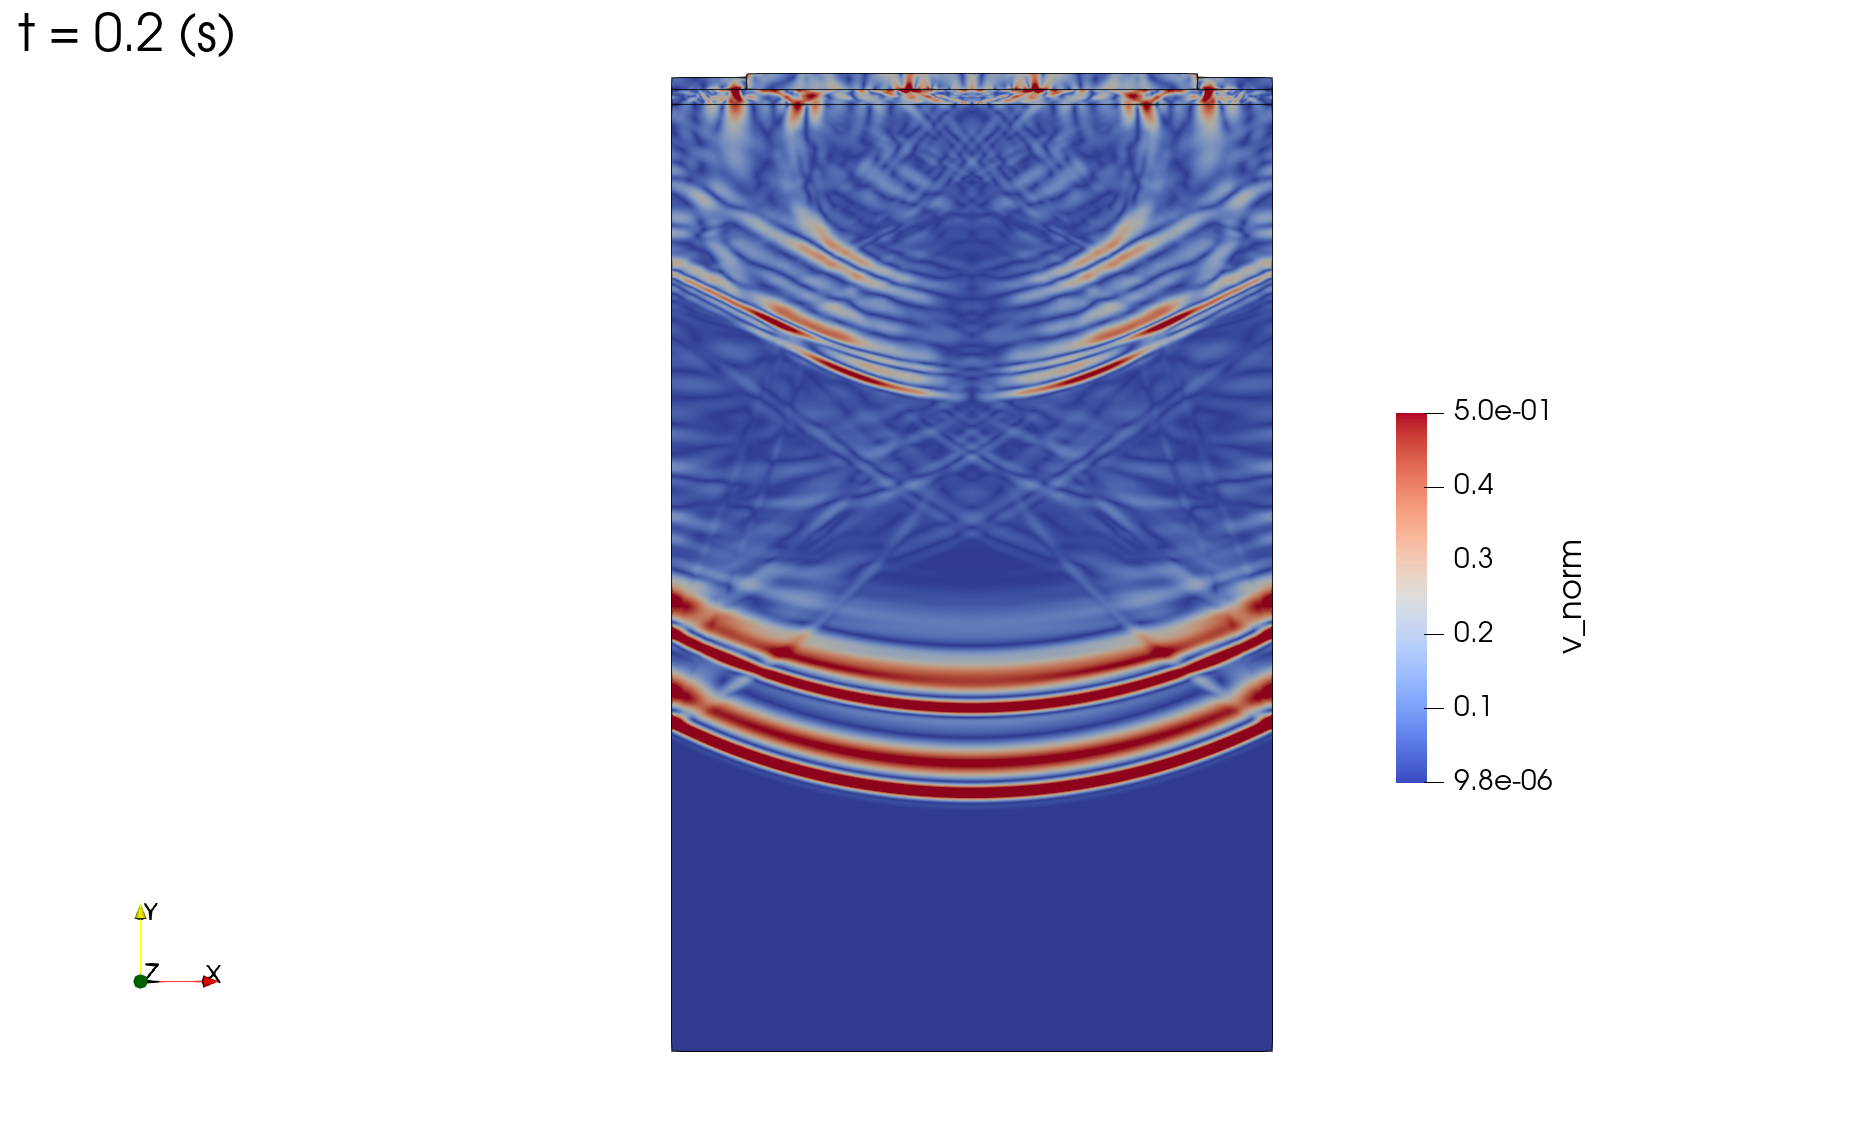
\includegraphics[trim={20cm 1cm 20cm 3cm},clip,width=0.32\textwidth]
    {images/gas_field/0.20.png}
    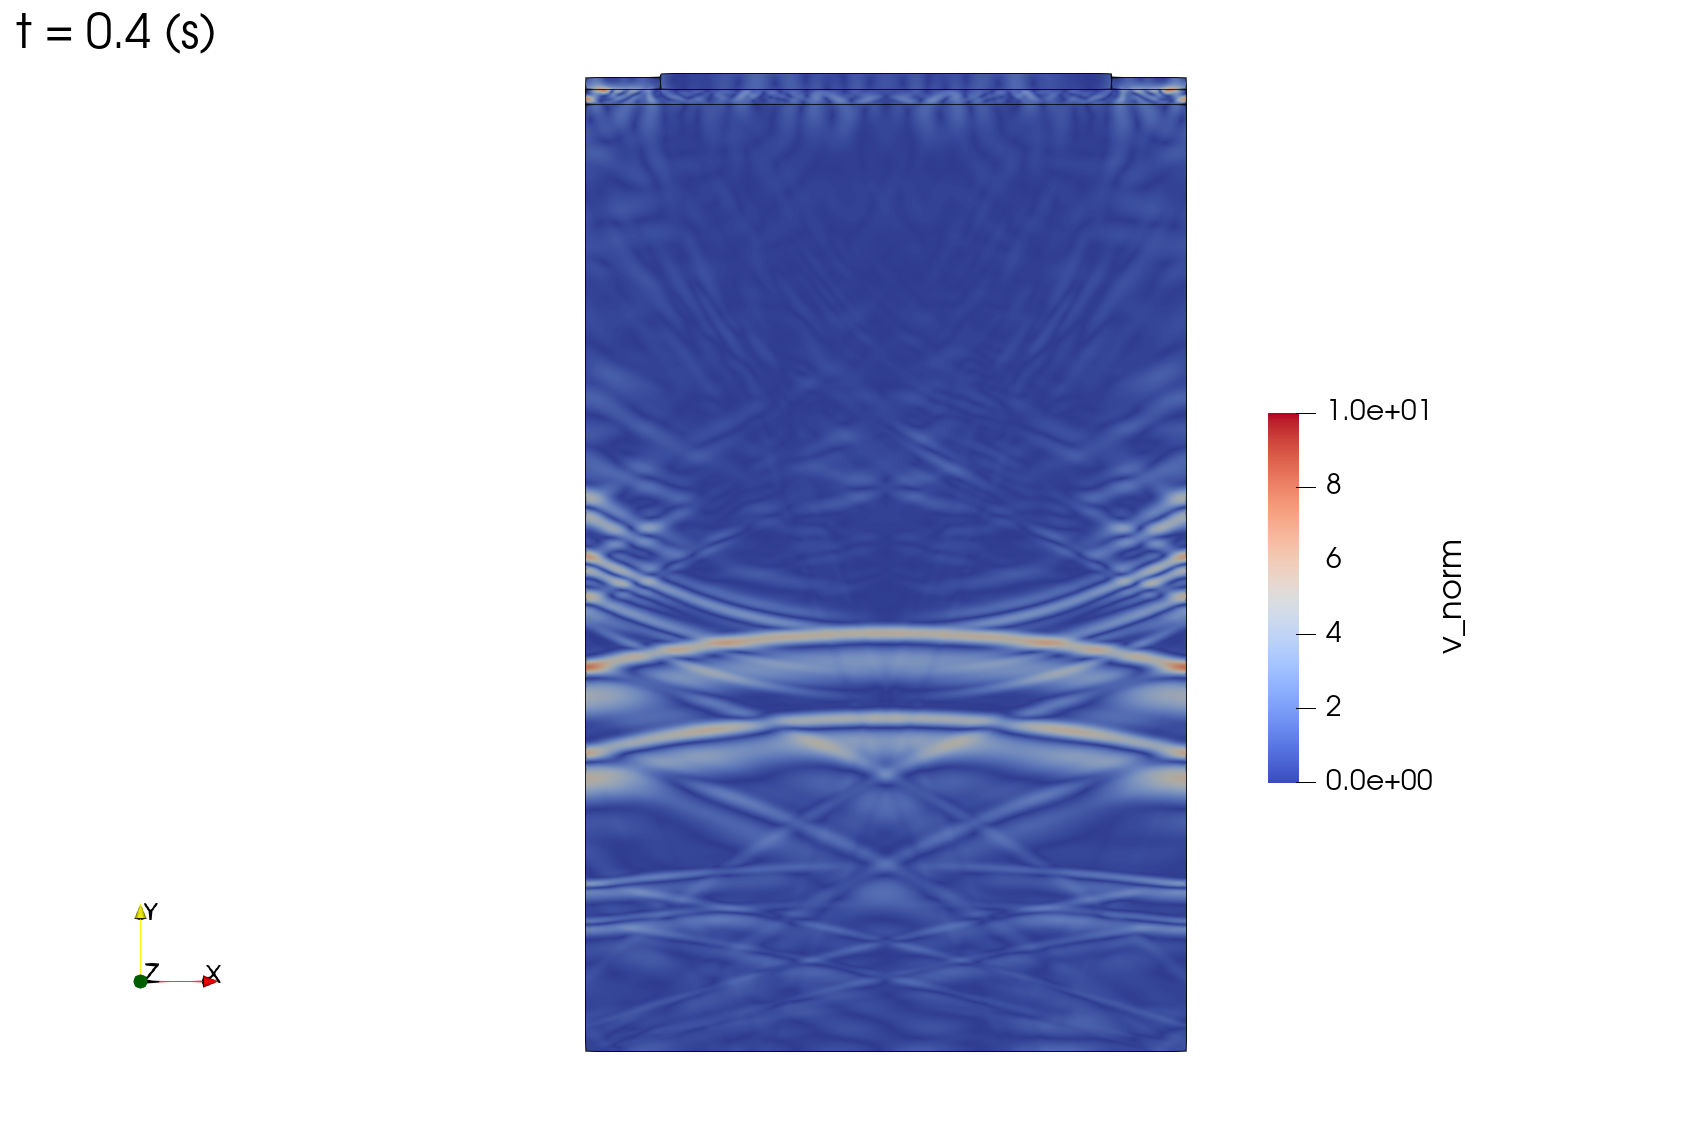
\includegraphics[trim={20cm 1cm 20cm 3cm},clip,width=0.32\textwidth]
    {images/gas_field/0.40.png}\\
    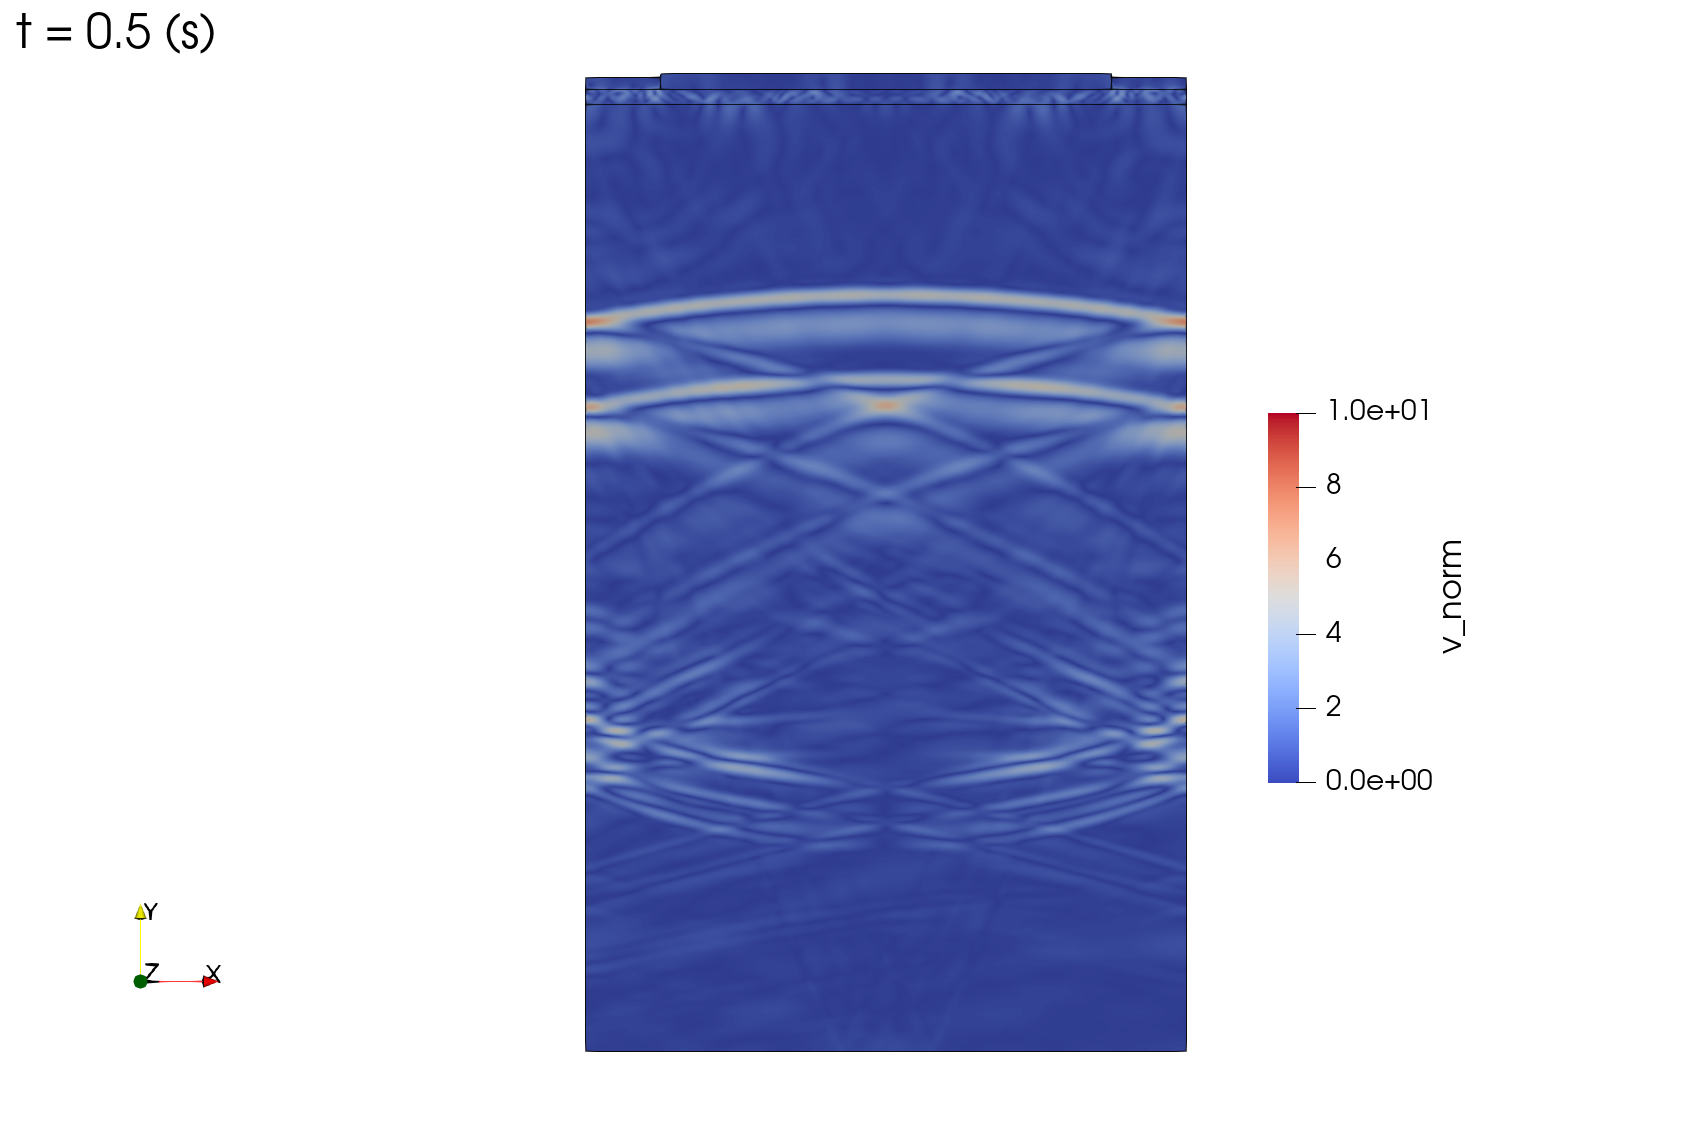
\includegraphics[trim={20cm 1cm 20cm 3cm},clip,width=0.32\textwidth]
    {images/gas_field/0.50.png}
    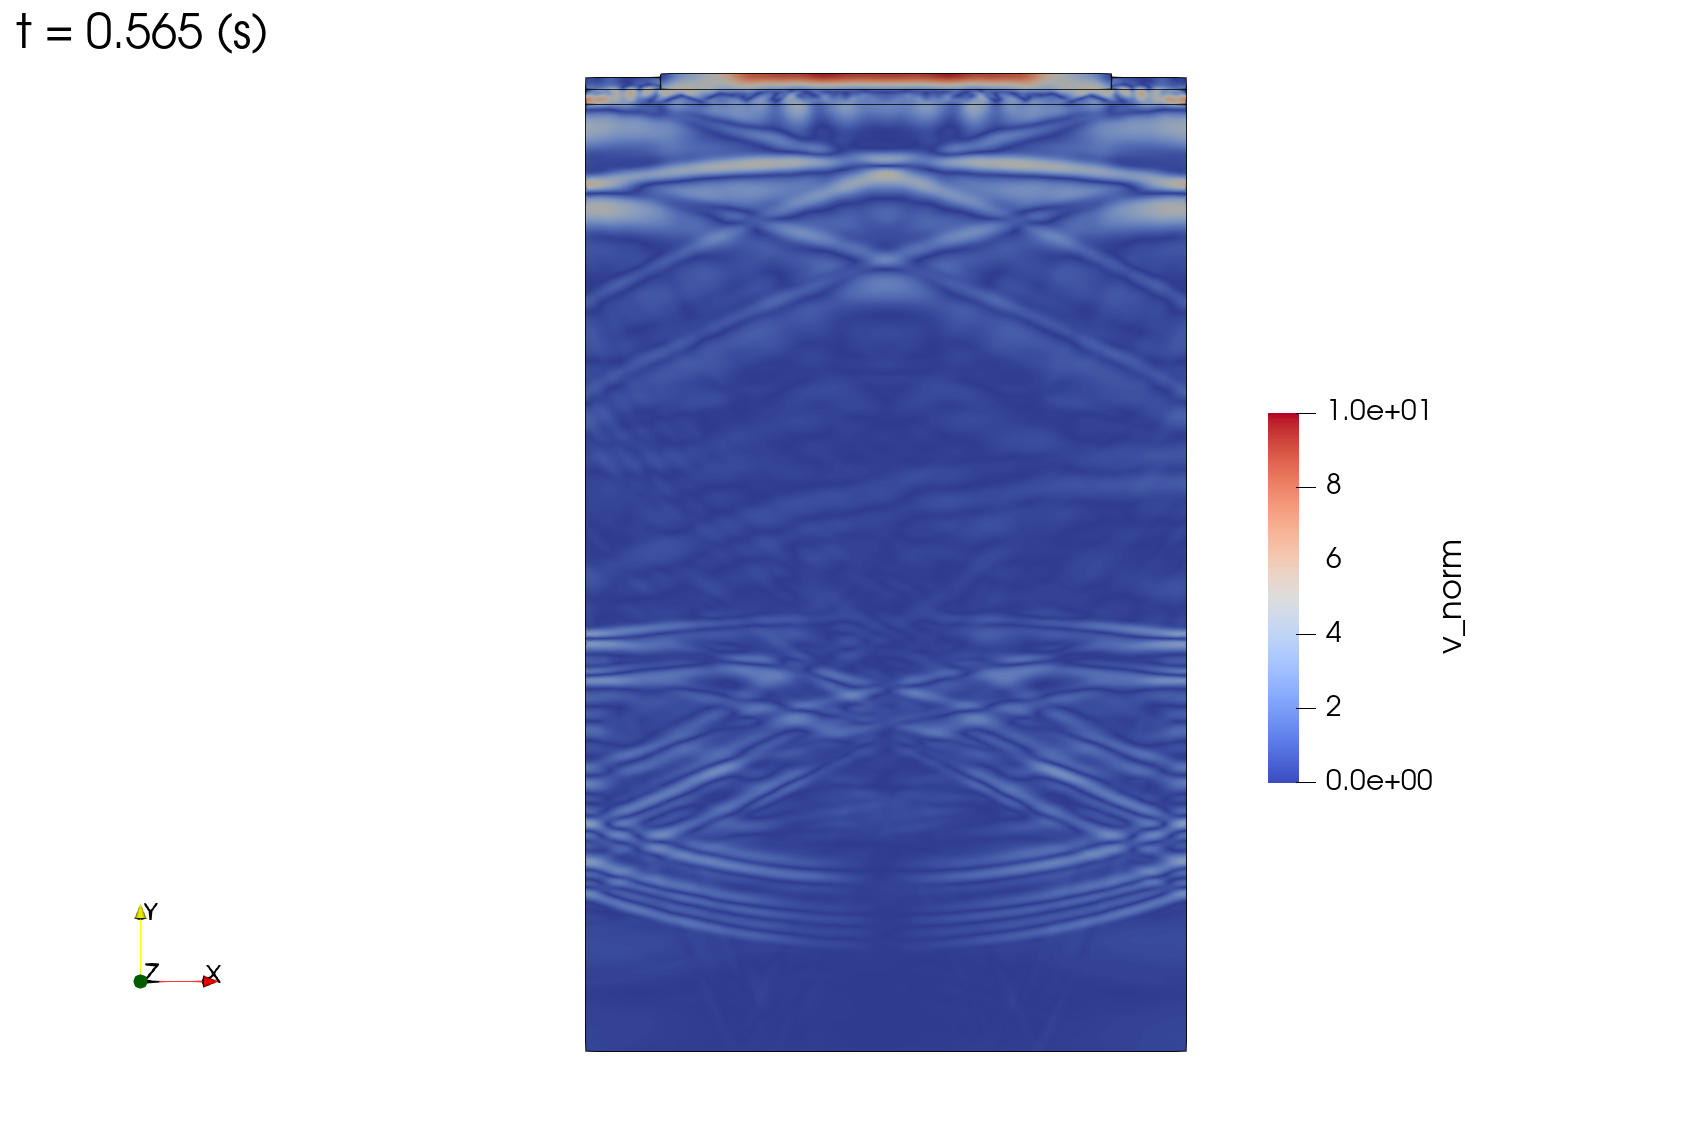
\includegraphics[trim={20cm 1cm 20cm 3cm},clip,width=0.32\textwidth]
    {images/gas_field/0.565.png}
    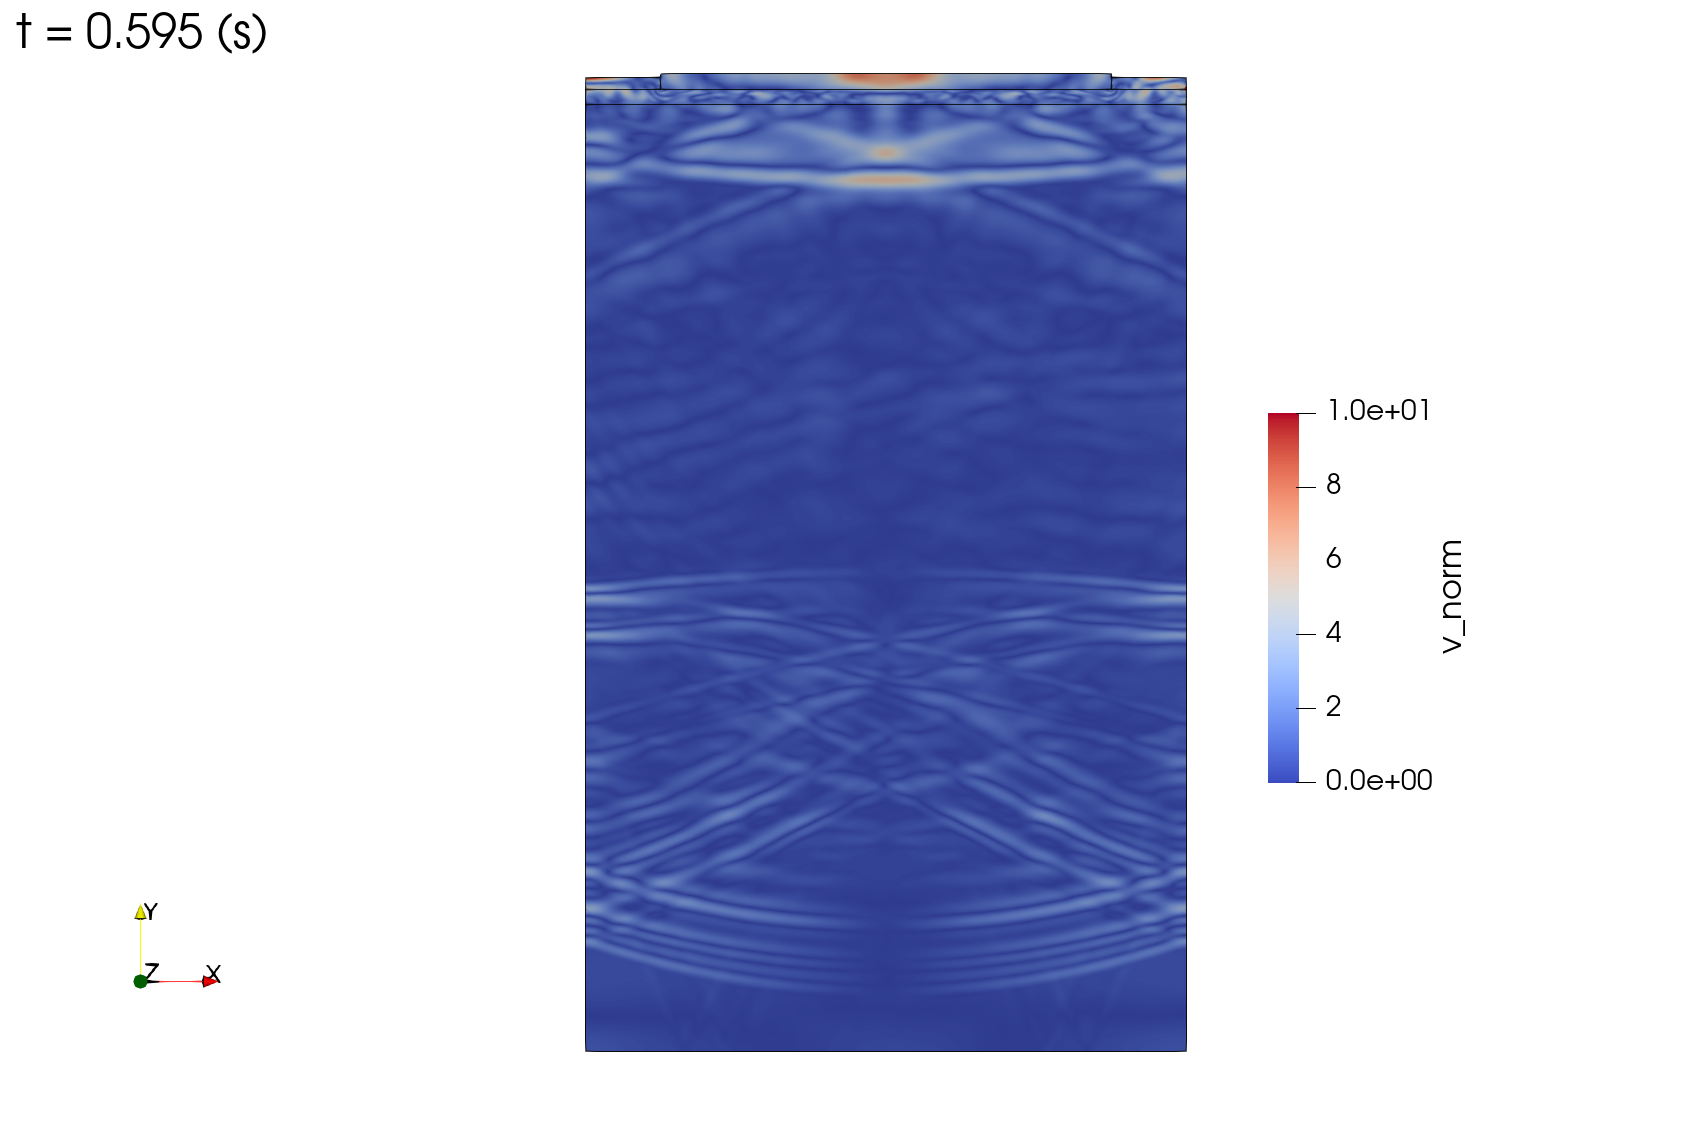
\includegraphics[trim={20cm 1cm 20cm 3cm},clip,width=0.32\textwidth]
    {images/gas_field/0.595.png}
    \caption{Волновая картина.}
    \label{fig:wave_image}
\end{figure}

\subsection{Моделирование статической нагрузки}



\input{3_abscorbing}

\section{Заключение}

В первой части данной работы было рассмотрено численное моделирование динамических процессов, происходящих в ледовом острове при бурении грунта и статической нагрузке острова. Анализ волновых картин, возникающих при моделировании бурения, показал, что ледовый остров проявляет свойства резонатора волн упругости. Это свидетельствует о наличии риска резонансного разрушения льда при наличии периодических источников возмущений вблизи острова. Также был проведён анализ распределений напряжений фон Мизеса в ледовом острове при 100-тонной статической нагрузке с 5-метровым основанием. Данная нагрузка оказалась недостаточной для разрушения льда. Наиболее нагруженными частями острова были цилиндрическая область непосредственно под основанием статической нагрузки, а также конусообразные области радиусом около 20 метров с вершиной в центре острова и вертикальной осью.

Во второй части данной работы была теоретически показана возможность применения поглощающих граничных условий типа Berenger PML и split-field PML совместно с сеточно-харак\-теристическим методом. Был поставлен и проведён численный эксперимент для сравнения эффективности сеточно-характеристических и конечно-разностных реализаций этих граничных условий, а также поглощающего граничного условия Mur. Анализ результатов показал превосходство сеточно-харак\-теристических реализаций PML методов над конечно-разностными. Также был предложен метод комбинирования граничных условий типов PML и Mur для улучшения качества поглощения. 

Полученные результаты могут быть использованы для решения задач об использовании искусственных ледовых островов и улучшения точности численного моделирования распространения упругих волн в задачах прикладной вычислительной геофизики.

\section*{Благодарности}
Я хотел бы поблагодарить своего научного руководителя профессора Игоря Борисовича Петрова за постановку  задачи и ценные обсуждения. Также я хотел бы поблагодарить Николая Игоревича Хохлова за оказанную помощь при исследовании поглощающих граничных условий.

\addcontentsline{toc}{section}{Благодарности}
\newpage

\printbibliography[heading=bibintoc]

\end{document}
